\documentclass{article}
% --- watermark (auto-inserted) ---
\usepackage{xcolor}
\usepackage{xfp}% \fpeval; in the kernel since 2022, harmless on older LaTeX
\usepackage{draftwatermark}
\newlength{\watermarkTextWidth}
\AddToHook{begindocument/end}{%
  \SetWatermarkText{\normalfont Generated by The Agentic Scientist}%
  \SetWatermarkFontSize{10pt}%
  \SetWatermarkLightness{0.85}%
  \settowidth{\watermarkTextWidth}{\normalfont\fontsize{10pt}{12pt}\selectfont Generated by The Agentic Scientist}%
  \edef\watermarkScale{\fpeval{0.8 * sqrt(\paperwidth**2 + \paperheight**2) / \watermarkTextWidth}}%
  \edef\watermarkAngle{\fpeval{atand(\paperheight/\paperwidth)}}%
  \SetWatermarkScale{\watermarkScale}%
  \SetWatermarkAngle{\watermarkAngle}%
}
% --- end watermark ---
 % For LaTeX2e
\usepackage{paper,times}

\usepackage{hyperref}
\usepackage{url}
\usepackage{graphicx}
\usepackage{booktabs}
\usepackage{amsmath,amssymb}
\usepackage{subcaption}

\title{A Five-Statistic Log-Linear Predictor of Random-Walk Cover Time on Small Connected Graphs: Measurements Against the $2m(n-1)$ Bound}
\author{Anonymous authors}

\begin{document}
\maketitle

\begin{abstract}
Worst-case bounds on the cover time of a simple random walk, such as $2m(n-1)$, are known to be loose for concrete small graphs. We ask whether five cheap, relabeling-invariant statistics (vertices, edges, mean degree, maximum degree, diameter) are enough to predict Monte Carlo start-averaged cover time more accurately than this bound on connected graphs with $6\le n\le 30$. We study a ridge regression from log-statistics to log cover time, fitted in-episode on 36 labelled synthetic graphs from 12 families and scored on 24 disjoint held-out graphs in a sealed evaluation. Its family-macro log mean absolute error is $0.181$, against $1.754$ for the bound, $0.870$ for a constant predictor, and $1.423$ when the same predictions are scored against shuffled targets; the median relative Monte Carlo standard error of the labels is $0.029$. The sealed evaluation completed with a qualified outcome. The evidence is narrow: two test graphs per family, a deterministic predictor whose three seeded episodes coincide, no uncertainty over graph draws, and no retained per-family errors, so the question of \emph{which graph types} the predictor fails on is left unanswered. The result characterises this sample of synthetic families and sizes; it does not establish reliability beyond them.
\end{abstract}

\section{Introduction}
The cover time of a connected undirected graph is the expected number of steps a simple random walk needs to visit every vertex. Classical analysis gives bounds in terms of the number of vertices $n$ and edges $m$: Aleliunas et al.\ \citep{Aleliunas1979RandomWU} showed that the cover time from any start is at most $2m(n-1)$, and Feige proved that no connected graph exceeds $(4/27+o(1))n^3$ and none falls below $(1+o(1))\,n\ln n$ \citep{Feige1995ATU,Feige1995ATL}. These statements are tight for extremal graphs, but they say little about what to expect for a particular small graph: the bound $2m(n-1)$ is tight up to a constant factor on some graphs such as paths and cycles, and on dense or well-connected graphs it overshoots by a factor that grows with $n$ (Section~\ref{sec:rationale}).

This paper studies a practical, measurable alternative. For connected graphs with $6\le n\le 30$, can a handful of cheap statistics (here $n$, $m$, mean degree, maximum degree and diameter), combined by a log-linear model fitted on a few dozen labelled graphs, predict cover time more accurately than the generic bound? A secondary question is how the prediction error depends on graph type. We answer the first question quantitatively within one sealed evaluation and state explicitly that the retained evidence does not answer the second.

\paragraph{What is studied.} The object is a deliberately simple reference predictor: standardised log-statistics, ridge regression, and a power-law reading of the result, $\widehat{C}\propto \prod_j s_j^{w_j}$. We claim no novelty for the model class. The contribution is a careful measurement: a sealed, content-disjoint evaluation with a pre-declared aggregation (family-macro mean of clipped log error), three baselines or controls scored under the same pipeline, a Monte Carlo noise-floor estimate for the labels, and an explicit accounting of what the evidence cannot support.

\paragraph{Contributions.}
\begin{itemize}
\item A precisely specified five-statistic log-linear ridge predictor for start-averaged cover time on connected graphs with $6\le n\le 30$, with an observation that three of its five features are exactly collinear, so the ridge penalty is structurally necessary (Section~\ref{sec:method}).
\item A sealed-evaluation measurement showing family-macro log MAE of $0.181$ for the predictor versus $1.754$ for the $2m(n-1)$ bound, $0.870$ for a constant predictor and $1.423$ for a shuffled-target control (Section~\ref{sec:results}).
\item A threats-to-validity analysis that separates what the evaluation supports (a large gap on this sample, large relative to the median Monte Carlo label noise) from what it does not (per-family reliability, uncertainty over graph draws, feature attribution, scaling beyond $n=30$) (Section~\ref{sec:discussion}).
\end{itemize}

\begin{figure}[t]
\centering
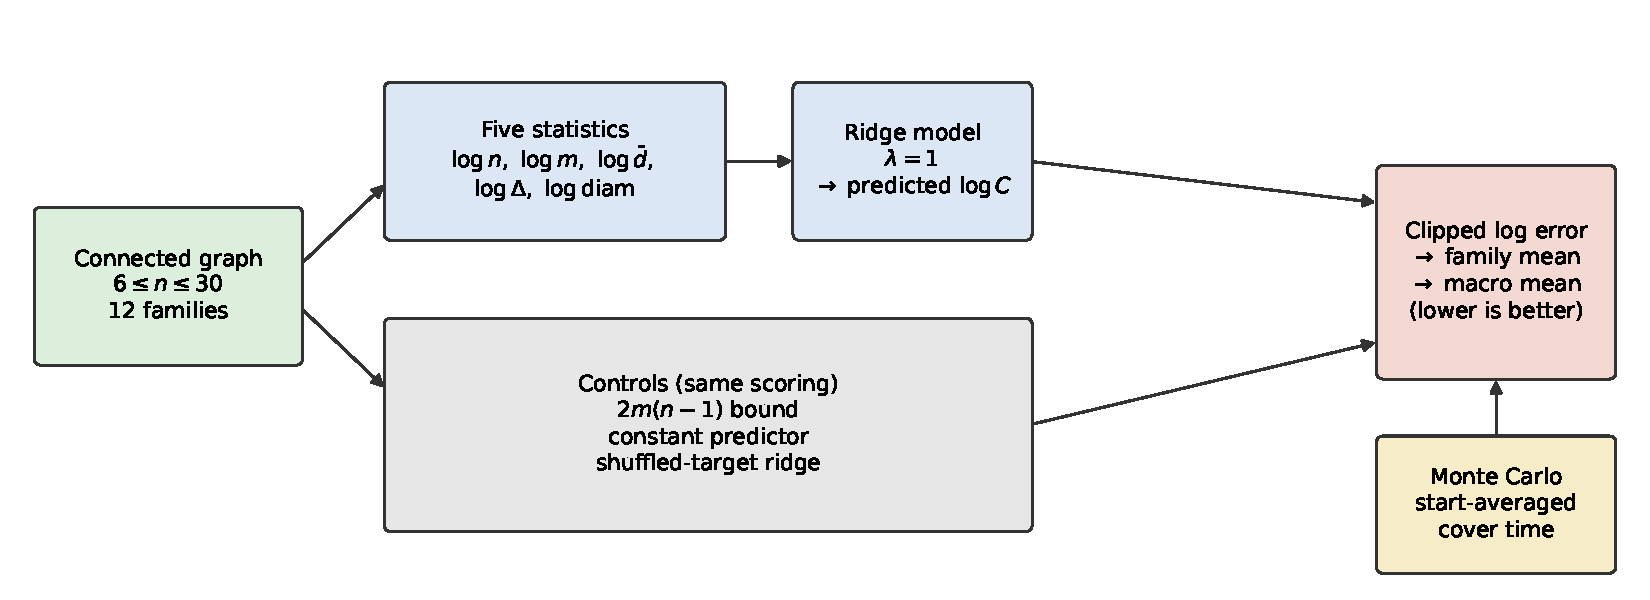
\includegraphics[width=\linewidth]{figures/overview_pipeline.pdf}
\caption{Overview of the study. A connected graph ($6\le n\le 30$) is reduced to five relabeling-invariant statistics; a ridge model predicts log cover time, which is compared with a Monte Carlo label. The $2m(n-1)$ bound, a constant predictor and a shuffled-target control are scored through the same pipeline: per-graph clipped log error $\rightarrow$ family mean $\rightarrow$ family-macro mean $\rightarrow$ mean over seeded episodes.}
\label{fig:overview}
\end{figure}

\section{Related Work}
\paragraph{Worst-case bounds.} The $2m(n-1)$ bound of Aleliunas et al.\ \citep{Aleliunas1979RandomWU} follows by summing commute times, each at most $2m$, over the $n-1$ edges of a spanning tree. Feige's upper bound, $(4/27+o(1))n^3$, is attained by lollipop-like graphs, and his companion lower bound, $(1+o(1))\,n\ln n$, is attained by the complete graph \citep{Feige1995ATU,Feige1995ATL}. Together these delimit the possible range of cover times for a given $n$ but are worst-case over all connected graphs; they are not intended as point predictions for a given graph. Lov\'asz's survey on random walks on graphs \citep{Lovasz2001RandomWO} collects the hitting-time and commute-time machinery behind such bounds, and the electrical-network view of random walks \citep{Doyle1984RandomWA} relates commute times to effective resistances. Our comparison against $2m(n-1)$ therefore measures how much a worst-case guarantee costs as a predictor on small graphs; it is not a criticism of the bound, which remains valid.

\paragraph{Cover times of specific models.} A complementary line of work derives the cover and hitting times of particular random-graph models, for example hyperbolic random graphs \citep{Kiwi2022CoverAH}. Such results exploit the generative structure of one model and give asymptotic statements. Our setting is different in three ways: the graphs form a mixture of twelve deterministic and random families, they are small, and the predictor is not told the family, so it must rely on statistics that are cheap to compute for any input graph.

\paragraph{Statistical prediction with cheap features.} Predicting a graph functional from low-dimensional summaries is a standard use of regression. What distinguishes this task is that the label is itself a Monte Carlo estimate with its own standard error, that the error is naturally multiplicative (cover times differ by orders of magnitude across graphs of similar size), and that the family composition of the test set drives the aggregate. We therefore work in log-space and aggregate over families rather than over graphs, so that a family with many graphs cannot dominate the score.

\section{Method}
\label{sec:method}

\subsection{Problem setup}
Let $G=(V,E)$ be a connected, undirected graph with $n=|V|$ and $m=|E|$. Let $C_v(G)$ be the expected number of steps for a simple random walk started at $v$ to visit all vertices, and let $C(G)=\frac1n\sum_{v}C_v(G)$ be the start-averaged cover time, which is the prediction target. A predictor receives a set of labelled training graphs (edges, a Monte Carlo estimate of $C(G)$ and its standard error) and unlabeled test graphs, and must return a finite positive prediction for every test graph. Vertex numbering and edge order carry no information: the evaluation sends randomly relabeled, edge-shuffled copies of the test graphs and requires predictions to agree to a relative tolerance of $10^{-6}$. % @evidence[[protocol_facts.json#PERM_TOL]]
Family names and test labels are never revealed to the predictor.

\paragraph{Success criterion.} For a test graph $g$ with Monte Carlo label $y_g$ and prediction $\hat y_g$, the per-graph error is $e_g=\min\!\big(|\ln(\hat y_g/y_g)|,\,10\big)$. The score is the family-macro log MAE: the mean of $e_g$ within each family, then the unweighted mean over the $12$ families, then the mean over three seeded episodes. Lower is better. A failed or malformed episode contributes the worst-case value of $10$, so the score cannot be improved by crashing. The same quantity is computed for the baselines below, so differences between rows are differences in prediction quality under one pipeline.

\subsection{Design rationale}
\label{sec:rationale}
Why should a few statistics help? The ratio between $2m(n-1)$ and the true cover time depends strongly on structure, and exactly solvable families make this concrete. Writing $H_k$ for the $k$-th harmonic number and $N=n-1$, the start-averaged cover times are: $C=N^2+N(N-1)/6$ on the path (with $m=N$); $C=n(n-1)/2$ on the cycle ($m=n$); $C=(n-1)H_{n-1}$ on the complete graph (a coupon-collector argument, $m=n(n-1)/2$); and $C=2NH_{N-1}+1/(N+1)$ on the star ($m=N$). We checked these closed forms against exact subset-dynamic-programming enumeration at $n=7$ (\texttt{scripts/verify\_closed\_forms.py}). % @evidence[[scripts/verify_closed_forms.py]]
Figure~\ref{fig:gap} plots the resulting log overshoot $\ln[2m(n-1)/C]$. On the path it is essentially constant, about $0.54$ at $n=30$; on the cycle it is exactly $\ln 4\approx1.39$ at every $n$; on the star it grows like $\ln(n/\ln n)$ to about $2.0$ at $n=30$; and on the complete graph it grows like $\ln(n^2/\ln n)$ to about $5.4$ at $n=30$. % @evidence[[closed_form_gap.json#log_overshoot]]
A single multiplicative constant therefore cannot repair the bound across families, because the required correction ranges over several nats within the studied size range. Exponents on $n$, $m$ and the diameter can in principle encode the structure that separates these regimes: dense graphs have large $m$ relative to $n$ and small diameter, path-like graphs have the opposite. The model should work to the extent that cover time on this graph population is approximately a power law in the statistics. Conversely, structurally different graphs can share all five statistics, which places a ceiling on what any function of these five numbers can achieve; we do not try to measure that ceiling. The closed-form curves cover only four of the twelve evaluated families and are not a prediction of the measured error of the bound on the test graphs.

\begin{figure}[t]
\centering
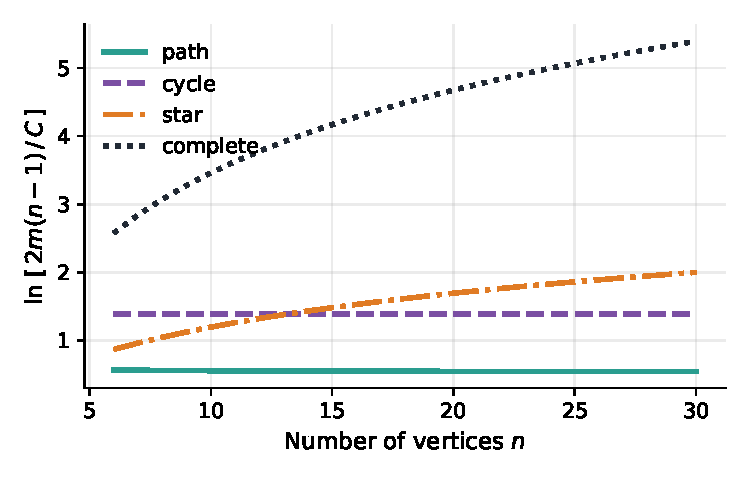
\includegraphics[width=0.7\linewidth]{figures/closed_form_gap.pdf}
\caption{Exact log overshoot $\ln[2m(n-1)/C]$ of the generic bound on four families with closed-form start-averaged cover times, for $6\le n\le 30$. The correction needed to turn the bound into a point prediction depends on the family and, for dense or star-like graphs, on $n$. These are analytic curves, not measurements.}
\label{fig:gap}
\end{figure}

\subsection{Compared predictors}
\paragraph{Five-statistic ridge predictor (studied).} For a graph with maximum degree $\Delta$, diameter $D$ (at least $1$) and mean degree $\bar d=2m/n$, the feature vector is
\[
x(G)=\big(\ln n,\ \ln m,\ \ln \bar d,\ \ln\Delta,\ \ln D\big).
\]
Features are standardised with the mean and (population) standard deviation of the training graphs. Writing $Z$ for the standardised training matrix, $y$ for the log Monte Carlo targets and $\bar y$ for their mean, the weights are
\[
w=\big(Z^\top Z+\lambda I\big)^{-1}Z^\top(y-\bar y),\qquad \lambda=1,
\]
with the intercept $\bar y$ unpenalised, and the prediction is $\hat y(G)=\exp\!\big(\bar y+z(G)^\top w\big)$ for the standardised feature $z(G)$. Because the model is linear in log-features it is a power law, $\hat y\propto n^{a_1}m^{a_2}\bar d^{a_3}\Delta^{a_4}D^{a_5}$. Since $\bar d=2m/n$, we have $\ln m=\ln n+\ln\bar d-\ln 2$ exactly, so the three features are linearly dependent and the design matrix has rank at most four; the ridge term is what makes the normal equations well posed and selects the minimum-norm solution in standardised coordinates. The model is refitted on all accumulated labelled graphs after each batch of training graphs. If no training graphs have been supplied, the implementation falls back to the bound itself; this safeguard is not part of the comparison.

\paragraph{Bound baseline.} The prediction is $2m(n-1)$ for every test graph, which requires no training data.

\paragraph{Constant baseline.} The prediction is the geometric mean of the training Monte Carlo targets, $\exp(\bar y)$, for every test graph. This is exactly the ridge model with all weights set to zero, so the ridge-versus-constant comparison is a controlled ablation of the entire feature set under an identical intercept.

\paragraph{Shuffled-target control.} The ridge predictions are scored against test targets permuted across graphs by a fixed derangement. A predictor that tracked the targets because of an artefact of the metric, rather than of graph structure, would score similarly under this control; the control therefore calibrates how large the metric is when predictions carry no information about the matched labels.

\subsection{Reading the model and the metric}
\label{sec:reading}
\paragraph{Effective parameterisation.} Because $\ln m=\ln n+\ln\bar d-\ln 2$, the five-feature power law is equivalent to a four-parameter family in $(\ln n,\ln \bar d,\ln\Delta,\ln D)$; the ridge solution distributes the shared signal over the three collinear features in the minimum-norm way. Individual fitted weights on $n$, $m$ and $\bar d$ are therefore not separately interpretable, and we do not interpret them. Only the fitted function (the prediction) is meaningful.

\paragraph{Why log error.} Cover times in this size range span orders of magnitude, and the relevant question for a practitioner is a multiplicative one: is the prediction within a factor of $e^{\epsilon}$ of the truth? The absolute log ratio treats over- and under-prediction symmetrically, is invariant to the units of the label, and is directly comparable between the predictor and the bound, whose predictions are on the label scale. Clipping at $10$ (a factor of $e^{10}\approx2.2\times10^{4}$) only limits the influence of catastrophic outputs.

\paragraph{Why family-macro aggregation.} The score averages graphs within a family first and then averages the $12$ family means with equal weight. This prevents a family with more or larger graphs from dominating the score and puts the structurally extreme families (path, lollipop, barbell) on the same footing as benign ones. The price is variance: with two test graphs per family, each family mean is a mean of two terms, and the score is sensitive to individual graphs.

\subsection{Experimental protocol}
\label{sec:protocol}
\paragraph{Graphs and labels.} Graphs are synthesised by code from twelve families: path, cycle, star, complete, grid, complete bipartite, barbell, lollipop, binary tree, random tree, Erd\H{o}s--R\'enyi, and random regular. The sealed evaluation uses $36$ labelled training graphs ($3$ per family, $6\le n\le 30$) and $24$ test graphs ($2$ per family, $8\le n\le 26$). % @evidence[[protocol_facts.json#final_train]] @evidence[[protocol_facts.json#final_test]]
Test graphs are content-hash disjoint from the graphs visible during model selection. Labels are Monte Carlo estimates of $C(G)$ computed by the evaluator from simple-random-walk simulations started equally often from every vertex, with about $300$ walks per graph in total; each label comes with a standard error. % @evidence[[protocol_facts.json#MC_WALKS]]
The evaluator's simulator is validated against exact cover times on small graphs before use.

\paragraph{Episodes and seeds.} The predictor is evaluated in three seeded episodes (seeds $201$, $202$, $203$); each episode resets all state, supplies the labelled graphs in batches of at most $16$, and requests predictions for the test graphs. % @evidence[[paper_data.json#final_evaluation.evaluation_evidence.episodes]]
The seeds control only the predictor's internal randomness; the graphs and Monte Carlo labels are fixed across episodes. The predictor uses no randomness, so the episodes are expected to coincide (Section~\ref{sec:results}).

\paragraph{Reporting.} All reported numbers come from the sealed evaluation record. We report the family-macro log MAE for each predictor, the median relative standard error $\mathrm{SE}_g/y_g$ of the test labels, and the maximum relative deviation of predictions across relabeled copies. We do not report per-graph or per-family errors because the retained record does not contain them, and we do not report a confidence interval over graph draws because none was computed. Selection context (how the studied configuration was fixed) is given in the Supplementary Information and does not enter the main comparison.

\subsection{Implementation}
The predictor is a self-contained Python module of about $140$ lines implementing the reset/fit/predict interface using only the standard library: breadth-first search from every vertex gives the diameter; a small Gaussian elimination with partial pivoting solves the five-by-five ridge system. Predictions are clipped from below at $10^{-9}$ to remain positive. The only hyper-parameter is $\lambda=1$, a fixed constant in the source that was not tuned on the sealed graphs. Source locations are listed in the Supplementary Information.

\section{Results}
\label{sec:results}

\subsection{Main comparison}
Table~\ref{tab:main} and Figure~\ref{fig:main} report the sealed-evaluation scores. The five-statistic ridge predictor attains a family-macro log MAE of $0.181$ % @evidence[[paper_data.json#final_evaluation.metrics.macro_log_mae]]
whereas the $2m(n-1)$ bound attains $1.754$, % @evidence[[paper_data.json#final_evaluation.metrics.bound_macro_log_mae]]
a difference of $1.572$. % @evidence[[paper_data.json#final_evaluation.metrics.improvement_vs_bound]]
Exponentiating the family-macro log MAE gives a rough geometric-average multiplicative error factor of $1.20$ for the predictor and $5.78$ for the bound; this conversion is arithmetic on the family-macro mean and is not a per-graph guarantee. The constant predictor scores $0.870$ % @evidence[[paper_data.json#final_evaluation.metrics.const_macro_log_mae]]
and the shuffled-target control $1.423$, % @evidence[[paper_data.json#final_evaluation.metrics.shuffle_macro_log_mae]]
so the ridge error is about one fifth of the constant error and about one tenth of the bound error (ratios $4.8$ and $9.7$; arithmetic on the reported values).

\begin{figure}[t]
\centering
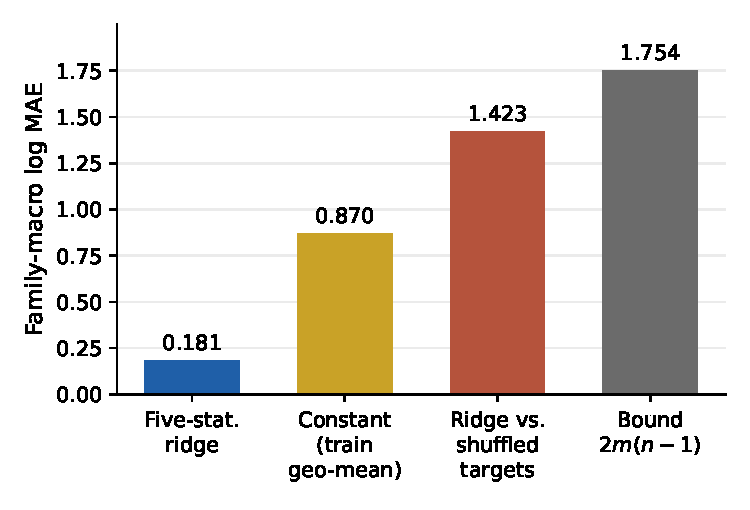
\includegraphics[width=0.7\linewidth]{figures/main_comparison.pdf}
\caption{Family-macro log MAE on the sealed held-out graphs (lower is better). The ridge predictor is compared with the $2m(n-1)$ bound, a constant predictor equal to the training geometric mean, and the ridge predictions scored against shuffled targets. Each bar is one evaluator-computed value; no error bars are shown because no uncertainty over graph draws was computed.}
\label{fig:main}
\end{figure}

\begin{table}[t]
\centering
\caption{Sealed-evaluation results. ``Factor'' is $\exp$ of the family-macro log MAE and ``Ratio'' is the log MAE divided by that of the ridge predictor; both are arithmetic conversions of the reported values.}
\label{tab:main}
\small
\begin{tabular}{lccc}
\toprule
Predictor / control & Family-macro log MAE & Factor & Ratio \\
\midrule
Five-statistic ridge & $0.181$ & $1.20$ & $1.0$ \\ % @evidence[[paper_data.json#final_evaluation.metrics.macro_log_mae]]
Constant (training geometric mean) & $0.870$ & $2.39$ & $4.8$ \\ % @evidence[[paper_data.json#final_evaluation.metrics.const_macro_log_mae]]
Ridge scored vs.\ shuffled targets & $1.423$ & $4.15$ & $7.8$ \\ % @evidence[[paper_data.json#final_evaluation.metrics.shuffle_macro_log_mae]]
Bound $2m(n-1)$ & $1.754$ & $5.78$ & $9.7$ \\ % @evidence[[paper_data.json#final_evaluation.metrics.bound_macro_log_mae]]
\bottomrule
\end{tabular}
\end{table}

\subsection{Controls and sanity checks}
\paragraph{Constant control as feature ablation.} Because the constant predictor shares the ridge intercept, the drop from $0.870$ to $0.181$ is attributable, within this evaluation, to the five-statistic term as a whole. The evaluation does \emph{not} contain per-feature ablations, so it cannot say which statistics matter, whether the collinear triple $(n,m,\bar d)$ contributes beyond two of its members, or whether the diameter feature carries the gain. Those attributions would require experiments that were not performed.

\paragraph{Shuffled-target control.} Scoring the same predictions against permuted targets yields $1.423$, much larger than $0.181$ and comparable in magnitude to the bound's $1.754$. The low error of the ridge predictor is therefore not a property of the metric or of the label distribution alone: when predictions are decoupled from their graphs' labels, the metric is roughly eight times larger. That the shuffled control is worse than the constant predictor is unsurprising: a constant hedges near the centre of the log-label distribution, whereas permuted predictions keep the full spread of the ridge outputs and pair it with the wrong labels.

\paragraph{Invariance.} The maximum relative deviation between predictions on a test graph and on its relabeled, edge-shuffled copies is $0.0$, % @evidence[[paper_data.json#final_evaluation.metrics.perm_max_rel_dev]]
well inside the tolerance of $10^{-6}$. This is expected from a predictor that uses only $n$, $m$, degree and diameter, and it confirms that no vertex-ordering information leaks into predictions.

\subsection{Monte Carlo uncertainty}
The labels are Monte Carlo estimates. The median relative standard error over test graphs is $0.029$, % @evidence[[paper_data.json#final_evaluation.metrics.mc_rel_se_median]]
about $2.9\%$, or roughly one sixth of the ridge log MAE ($0.029/0.181\approx0.16$; arithmetic). The label noise is thus small relative to the prediction error and very small relative to the bound's error, and the headline gap cannot be explained by label noise. A simple calibration helps: if the predictor were exact and each label were perturbed by a Gaussian relative error with standard deviation equal to this median, the expected absolute log error would be $\sqrt{2/\pi}\times0.029\approx0.023$, about $13\%$ of the observed $0.181$. % @evidence[[closed_form_gap.json#noise_floor_mae_gaussian]]
This is an order-of-magnitude statement under a Gaussian approximation, not a measured noise floor, but it indicates that label noise explains only a minor part of the ridge error. Two cautions apply. First, this is a median: the retained record does not include the maximum standard error or the per-graph values, so the noisiest graphs (likely the slowest-covering families) may carry larger relative uncertainty. Second, the standard error treats the walks as independent samples of cover time and characterises only simulation noise; it does not include the variability of which graphs were drawn.

\subsection{Episode-level consistency}
The three seeded episodes each yield the same score, $-0.18137$ (the sign convention is that the score is the negated family-macro log MAE), with durations of roughly $0.06$ seconds each. % @evidence[[paper_data.json#final_evaluation.evaluation_evidence.episodes]]
This identity is the expected behaviour of a deterministic predictor evaluated on fixed graphs with fixed labels. It demonstrates reproducibility of the evaluation, not statistical stability: zero spread across episodes must not be read as zero uncertainty, because the only source of randomness varied across episodes (the predictor's seed) is not used by the predictor.

\subsection{Qualification status}
The sealed evaluation completed and its outcome is recorded as qualified. % @evidence[[paper_data.json#final_evaluation.outcome]]
The evaluation record also marks diagnostics reported by the candidate itself as unverified; we use none of them and rely only on the evaluator-computed metrics above. Because the outcome is qualified, there is no qualification failure to disclose or to attribute to performance or to validity. Qualification speaks to the completed, sealed measurement; it is not a claim of generalisation, validity beyond the evaluated sample, or superiority over any predictor other than those compared here.

\subsection{What the evidence does not show: error by graph type}
The second research question asks how error depends on graph type. The retained evaluation record reports only family-macro aggregates; per-family and per-size errors were not retained, and we do not attempt to reconstruct them. We can therefore not say that the predictor is reliable on, or fails on, any named family. The aggregation itself offers a bounded statement: since the score is an unweighted mean over $12$ families, a macro value of $0.181$ means the average family-level mean log error is $0.181$, and this is compatible with a mix of families with small errors and a few with larger ones. Which of these holds remains unknown. Arithmetic does give a loose bound: since errors are non-negative, no family mean can exceed $12\times0.181\approx2.18$ (a multiplicative factor of about $8.8$), and, with two test graphs per family, no single graph's log error can exceed $24\times0.181\approx4.35$ (a factor of about $78$). % @evidence[[closed_form_gap.json#worst_case_family_mean_log_error]]
These worst-case concentrations are far from informative about where the error actually lies, but they show that the macro value alone already excludes a predictor that is catastrophically wrong on many families.

\section{Discussion and Limitations}
\label{sec:discussion}
\paragraph{What the result supports.} Within one sealed evaluation of $24$ held-out graphs from $12$ synthetic families with $8\le n\le 26$, a log-linear model on five cheap statistics tracks Monte Carlo cover times with family-macro log error of $0.181$, far below the $2m(n-1)$ bound ($1.754$), the constant predictor ($0.870$) and the shuffled-target control ($1.423$). The gap to the bound is large relative to Monte Carlo label noise.

\paragraph{Small test set and composition.} Each family contributes only two test graphs, and families are weighted equally regardless of size or variability. A single mis-predicted graph shifts its family mean by half of that graph's error and the macro mean by one twenty-fourth of it. The test set includes extremal families (lollipop, barbell, path) as well as well-connected ones (complete, random regular), which is useful for contrast, but the sample is not a draw from any natural population of graphs. The result describes this mixture and nothing else.

\paragraph{No uncertainty over graph draws.} The only uncertainty reported is Monte Carlo label noise. We did not bootstrap over test graphs, resample training sets, or generate repeated graph draws, so we cannot give a confidence interval for the macro log MAE. The apparent determinism across episodes is not a substitute.

\paragraph{Training-set size.} The model is fitted on $36$ labelled graphs (three per family) with five features of rank four; the ridge penalty $\lambda=1$ is a fixed constant. Whether the result is sensitive to $\lambda$, to training-set size or to the composition of the training families was not measured.

\paragraph{Feature attribution and ceiling.} We do not know which features carry the gain, nor how close a function of these five statistics can get to the label: structurally different graphs can share all five statistics. Richer invariants (for instance, effective-resistance quantities motivated by the relation between commute times and resistances \citep{Doyle1984RandomWA,Lovasz2001RandomWO}) are natural candidates, but a configuration of that kind produced no score in this study and we draw no conclusion about it.

\paragraph{Range of validity.} All graphs have $n\le 30$ and are drawn from twelve named families; labels are start-averaged, not worst-case-start, cover times. Extrapolation to larger graphs, to other families (e.g.\ scale-free or hyperbolic random graphs \citep{Kiwi2022CoverAH}) or to the maximum over start vertices is untested. A power-law fit calibrated at $n\le 30$ has no guarantee at larger $n$ and, in particular, should not be expected to respect the extremal exponents known from \citet{Feige1995ATU}.

\paragraph{Evaluation scope and label noise.} Per-graph Monte Carlo standard errors were not retained, so the noise on the slowest-covering graphs cannot be assessed here, and per-graph and per-family errors were not retained. The clip at $10$ on the per-graph log error cannot have been binding: the family-macro value of $0.181$ bounds every single test graph's error at about $4.35$ (a factor of about $78$).

\paragraph{Summary of what is and is not established.} Table~\ref{tab:status} separates the statements that the evidence supports from those it does not.

\begin{table}[t]
\centering
\caption{Status of the statements a reader might want to draw from this study.}
\label{tab:status}
\small
\begin{tabular}{p{0.52\linewidth}p{0.38\linewidth}}
\toprule
Statement & Status \\
\midrule
Ridge predictor has lower family-macro log MAE than the $2m(n-1)$ bound on the sealed graphs & Supported ($0.181$ vs.\ $1.754$) \\
Gain comes from the five-statistic term rather than the intercept or the metric & Supported by constant and shuffled controls, as a whole \\
Gap is not an artefact of label noise & Supported (median relative SE $0.029$) \\
Predictions are relabeling invariant & Supported (deviation $0.0$) \\
Which individual statistic drives the gain & Not tested \\
Which graph families are predicted well or badly & Unknown (not retained) \\
Confidence interval over graph draws & Not measured \\
Behaviour for $n>30$ or other families & Not tested \\
\bottomrule
\end{tabular}
\end{table}

\section{Conclusion}
For connected graphs with at most $30$ vertices, a ridge regression on five relabeling-invariant log-statistics predicted Monte Carlo start-averaged cover time with a family-macro log MAE of $0.181$ in a sealed evaluation, compared with $1.754$ for the generic $2m(n-1)$ bound, $0.870$ for a constant predictor, and $1.423$ when the predictions were scored against shuffled targets. Median relative Monte Carlo label error was $0.029$, small compared with the gap. The evaluation completed with a qualified outcome. In answer to the first research question, cheap statistics can give a markedly more accurate point prediction than the bound on this sample; in answer to the second, the retained evidence does not say on which graph types the predictor is reliable or fails. The most valuable next measurements are inexpensive and well-defined: per-family and per-size error reporting with Monte Carlo and graph-bootstrap uncertainty, per-feature ablations, sensitivity to the ridge penalty and training-set composition, and a comparison with richer invariants such as resistance-based features \citep{Doyle1984RandomWA}.

% IMPORTANT: \clearpage flushes all pending floats before references so that
% body-page counting excludes reference-only pages.  Do NOT remove.
\clearpage
\bibliography{references}
\bibliographystyle{paper}

\clearpage
\appendix
\section{Supplementary Information}

\subsection{Predictor specification and source locations}
The studied configuration is a single Python module; the table lists the elements that determine its predictions and where they are defined in the inspected source (\texttt{source\_evidence/downstream/program/src/program.py}). % @evidence[[source_evidence/downstream/program/src/program.py]]

\begin{table}[h]
\centering
\caption{Implementation elements of the five-statistic ridge predictor.}
\label{tab:impl}
\small
\begin{tabular}{p{0.28\linewidth}p{0.36\linewidth}p{0.26\linewidth}}
\toprule
Element & Setting & Source lines \\
\midrule
Feature vector & $\ln n,\ln m,\ln\bar d,\ln\Delta,\ln D$; $D\ge1$ & 75--82 \\
Ridge penalty & $\lambda=1$ on standardised features; intercept unpenalised & 49, 106--118 \\
Standardisation & training mean and population standard deviation (zero deviation replaced by $1$) & 106--112 \\
Linear solve & Gaussian elimination, partial pivoting & 89--103 \\
Prediction & $\max(\exp(\bar y+z^\top w),10^{-9})$ & 120--126 \\
No-training fallback & $2m(n-1)$ & 84--87, 122--123 \\
Refit rule & refit on all accumulated graphs after every fit call; reset clears state & 129--139 \\
\bottomrule
\end{tabular}
\end{table}

The specification file \texttt{program\_spec.toml} names \texttt{program.py} under \texttt{src} as the entry point and declares no additional integration settings. The inspected source of the studied configuration and of the reference configuration retained by model selection are identical.

\subsection{Evaluation protocol and split composition}
Table~\ref{tab:splits} gives the composition of the graph sets used by the sealed evaluation and, for context, by the selection procedure. % @evidence[[protocol_facts.json#final_train]] @evidence[[protocol_facts.json#search_train]]
Both use the same twelve families with an equal number of graphs per family within each split.

\begin{table}[h]
\centering
\caption{Graph-set composition. ``Per family'' is the number of graphs from each of the twelve families.}
\label{tab:splits}
\small
\begin{tabular}{llccc}
\toprule
Use & Split & Graphs & Per family & $n$ range \\
\midrule
Sealed evaluation & training & 36 & 3 & 6--30 \\
Sealed evaluation & held-out test & 24 & 2 & 8--26 \\
Selection & training & 24 & 2 & 6--26 \\
Selection & test & 12 & 1 & 9--16 \\
\bottomrule
\end{tabular}
\end{table}

Aggregation is fixed before evaluation with equal weights: per-graph error $\min(|\ln(\hat y/y)|,10)$, mean within family, unweighted mean over families, mean over episodes. A failed episode would contribute $10$ to the macro error and a perturbation deviation of $10^{6}$; none is recorded here. Monte Carlo labels simulate walks from every start vertex equally often, about $300$ walks per graph in total (run-time \texttt{MC\_WALKS}$=300$), with the standard error computed from the sample standard deviation of observed cover times. % @evidence[[protocol_facts.json#MC_WALKS]] @evidence[[protocol_facts.json#ERR_CLIP]]

\subsection{Episode records and qualification}
\begin{table}[h]
\centering
\caption{Per-episode records from the sealed evaluation (score is the negated family-macro log MAE).}
\label{tab:episodes}
\small
\begin{tabular}{lcc}
\toprule
Seed & Score & Duration (s) \\
\midrule
201 & $-0.18137$ & $0.058$ \\ % @evidence[[paper_data.json#final_evaluation.evaluation_evidence.episodes]]
202 & $-0.18137$ & $0.056$ \\
203 & $-0.18137$ & $0.060$ \\
\bottomrule
\end{tabular}
\end{table}

The evaluation status is completed and the qualification outcome is qualified. % @evidence[[paper_data.json#final_evaluation.outcome]]
Candidate-reported diagnostics are marked unverified in the evaluation record; they are not used. The evaluation record exposes no gate-level diagnostics, so we make no statement about which individual criteria were checked beyond the overall outcome.

\subsection{Selection context (separate from the sealed result)}
The configuration studied here is the reference configuration retained by model selection. The selection procedure considered one alternative candidate, a resistance-calibrated Matthews-style predictor, and it produced no score: zero candidates were scored and one was unscored. % @evidence[[paper_data.json#downstream_study.attempt_counts]]
Unscored candidates are missing evidence rather than measured losses, and we draw no conclusion about that alternative. The selection score of the retained configuration was $-0.1913$ (a negated macro log MAE on the selection test graphs), identical to the reference by construction, so the score difference is $0.0$. % @evidence[[paper_data.json#downstream_study.baseline_score]] @evidence[[paper_data.json#downstream_study.search_score_delta]]
Selection scores and sealed-evaluation scores come from different graph sets and different labels, and are not comparable; in particular, $0.191$ versus $0.181$ must not be read as an improvement or a degradation.

\subsection{Reproduction notes}
The predictor needs only a Python 3 interpreter with the standard library. The evaluation harness supplies the Monte Carlo labels and seeds; the reported seeds are $201$, $202$ and $203$. The scripts \texttt{scripts/build\_figures.py} and \texttt{scripts/extract\_protocol.py} regenerate Figure~\ref{fig:main} and the protocol facts used in this paper from the evaluation record and the task resources; the former requires matplotlib. % @evidence[[scripts/build_figures.py]] @evidence[[scripts/extract_protocol.py]]

\subsection{LLM Usage}
Large language models were used in this work as research and writing assistants. They proposed candidate predictors for the study, implemented and ran the experiments through an automated research pipeline, and drafted and edited this manuscript from the recorded evaluation artifacts. All reported numbers were taken from the evaluation record and checked against it; responsibility for the content rests with the submitting authors.

\end{document}
